\section{The Puzzle of Fast \& Useful Transfer}\label{sec:useful-transfer}
 
In this section, we relate the convergence rate of optimal HPs (e.g., learning rate) to that of the evaluation metric (e.g., validation loss). 
As previously discussed, the definition of weak transfer ensures that $\bhp^\star(n) \to \bhp^\star(\infty)$, but we need to characterize the rate of convergence in order to conclude the computational efficiency of the transfer strategy. As we will see in Proposition \ref{prop:basic_rate}, the convergence rate of $\phi_n \to \phi_\infty$ already implies an upper bound on the convergence rate of the minimizers $\bhp^\star(n)$ due to the local strong convexity condition of $\phi_\infty$. Moreover, it turns out that this convergence also informs whether it is computationally more efficient to use HP transfer than to directly tune the model at a single width $n$, as we show in Theorem \ref{thm:grid_and_transfer_rate}. We then present toy examples where the convergence rates of the optimal HP and loss can be quantified. 

\subsection{Convergence Rates of HP Transfer}\label{sec:hp-asymptotics}

\paragraph{Notation.}
Given deterministic sequences $x_n \in \mathbb{R}$ and $y_n \in \mathbb{R}^+$, we write $x_n = O(y_n)$ to mean there exists $c > 0$ such that $|x_n| \leq c y_n$ for all large $n$. We write $x_n = o(y_n)$ if $x_n / y_n \to 0$ as $n \to \infty$, and $x_n = \Theta(y_n)$ if there exist $c_1, c_2 > 0$ such that $c_1 y_n \leq |x_n| \leq c_2 y_n$ for all large $n$. As shorthand, we write $x_n \sim y_n$ to mean $x_n = \Theta(y_n)$. We overload the same notation for random quantities: whenever $x_n$ is random, $O(\cdot)$, $o(\cdot)$, $\Theta(\cdot)$, and $\sim$ are understood in the corresponding stochastic sense (i.e., $O_p$, $o_p$, $\Theta_p$), and limits $x_n \to x$ are interpreted as convergence in probability unless stated otherwise \citep[Section~2.2]{vandervaart1998asymptotic}.


\paragraph{Tracking the Width Dependence.}
We now introduce three quantities that track the convergence of the optimal loss and HPs, illustrated in Figure~\ref{fig:convergent-quantities}.

\begin{definition}[Convergent Quantities] \label{def:convergent_quantities}
We define the following width-dependent quantities.
    \begin{itemize}[leftmargin=*] 
    \item \textbf{Loss gap:} $a_n = |\phi_n^\star - \phi_\infty^\star|$. The quantity measures the discrepancy between the optimal value of the metric $\phi$ at the finite-width model (over all HPs) and that of the infinite-width model.
    \item \textbf{Hyperparameter gap:} $b_n = \norm{\bhp^\star(n) - \bhp^\star(\infty)}$. The quantity measures the discrepancy between the optimal HPs at width $n$ and the infinite-width counterpart.
    
    \item \textbf{Transfer suboptimality gap:} $c_n = |\phi_\infty(\bhp^\star(n)) - \phi_\infty^\star|$. The quantity measures the performance gap between two infinite-width models: one with the optimal HP tuned at infinite-width, and the other with the optimal HP at a smaller width. 
    Intuitively speaking, this quantity reflects the performance gap in transferring the optimal HP in a small model to a large model. 
\end{itemize}
\end{definition} 

\begin{figure}[t]
% \vspace{-2mm} 
\centering
\begin{minipage}[t]{0.32\linewidth}
\centering
{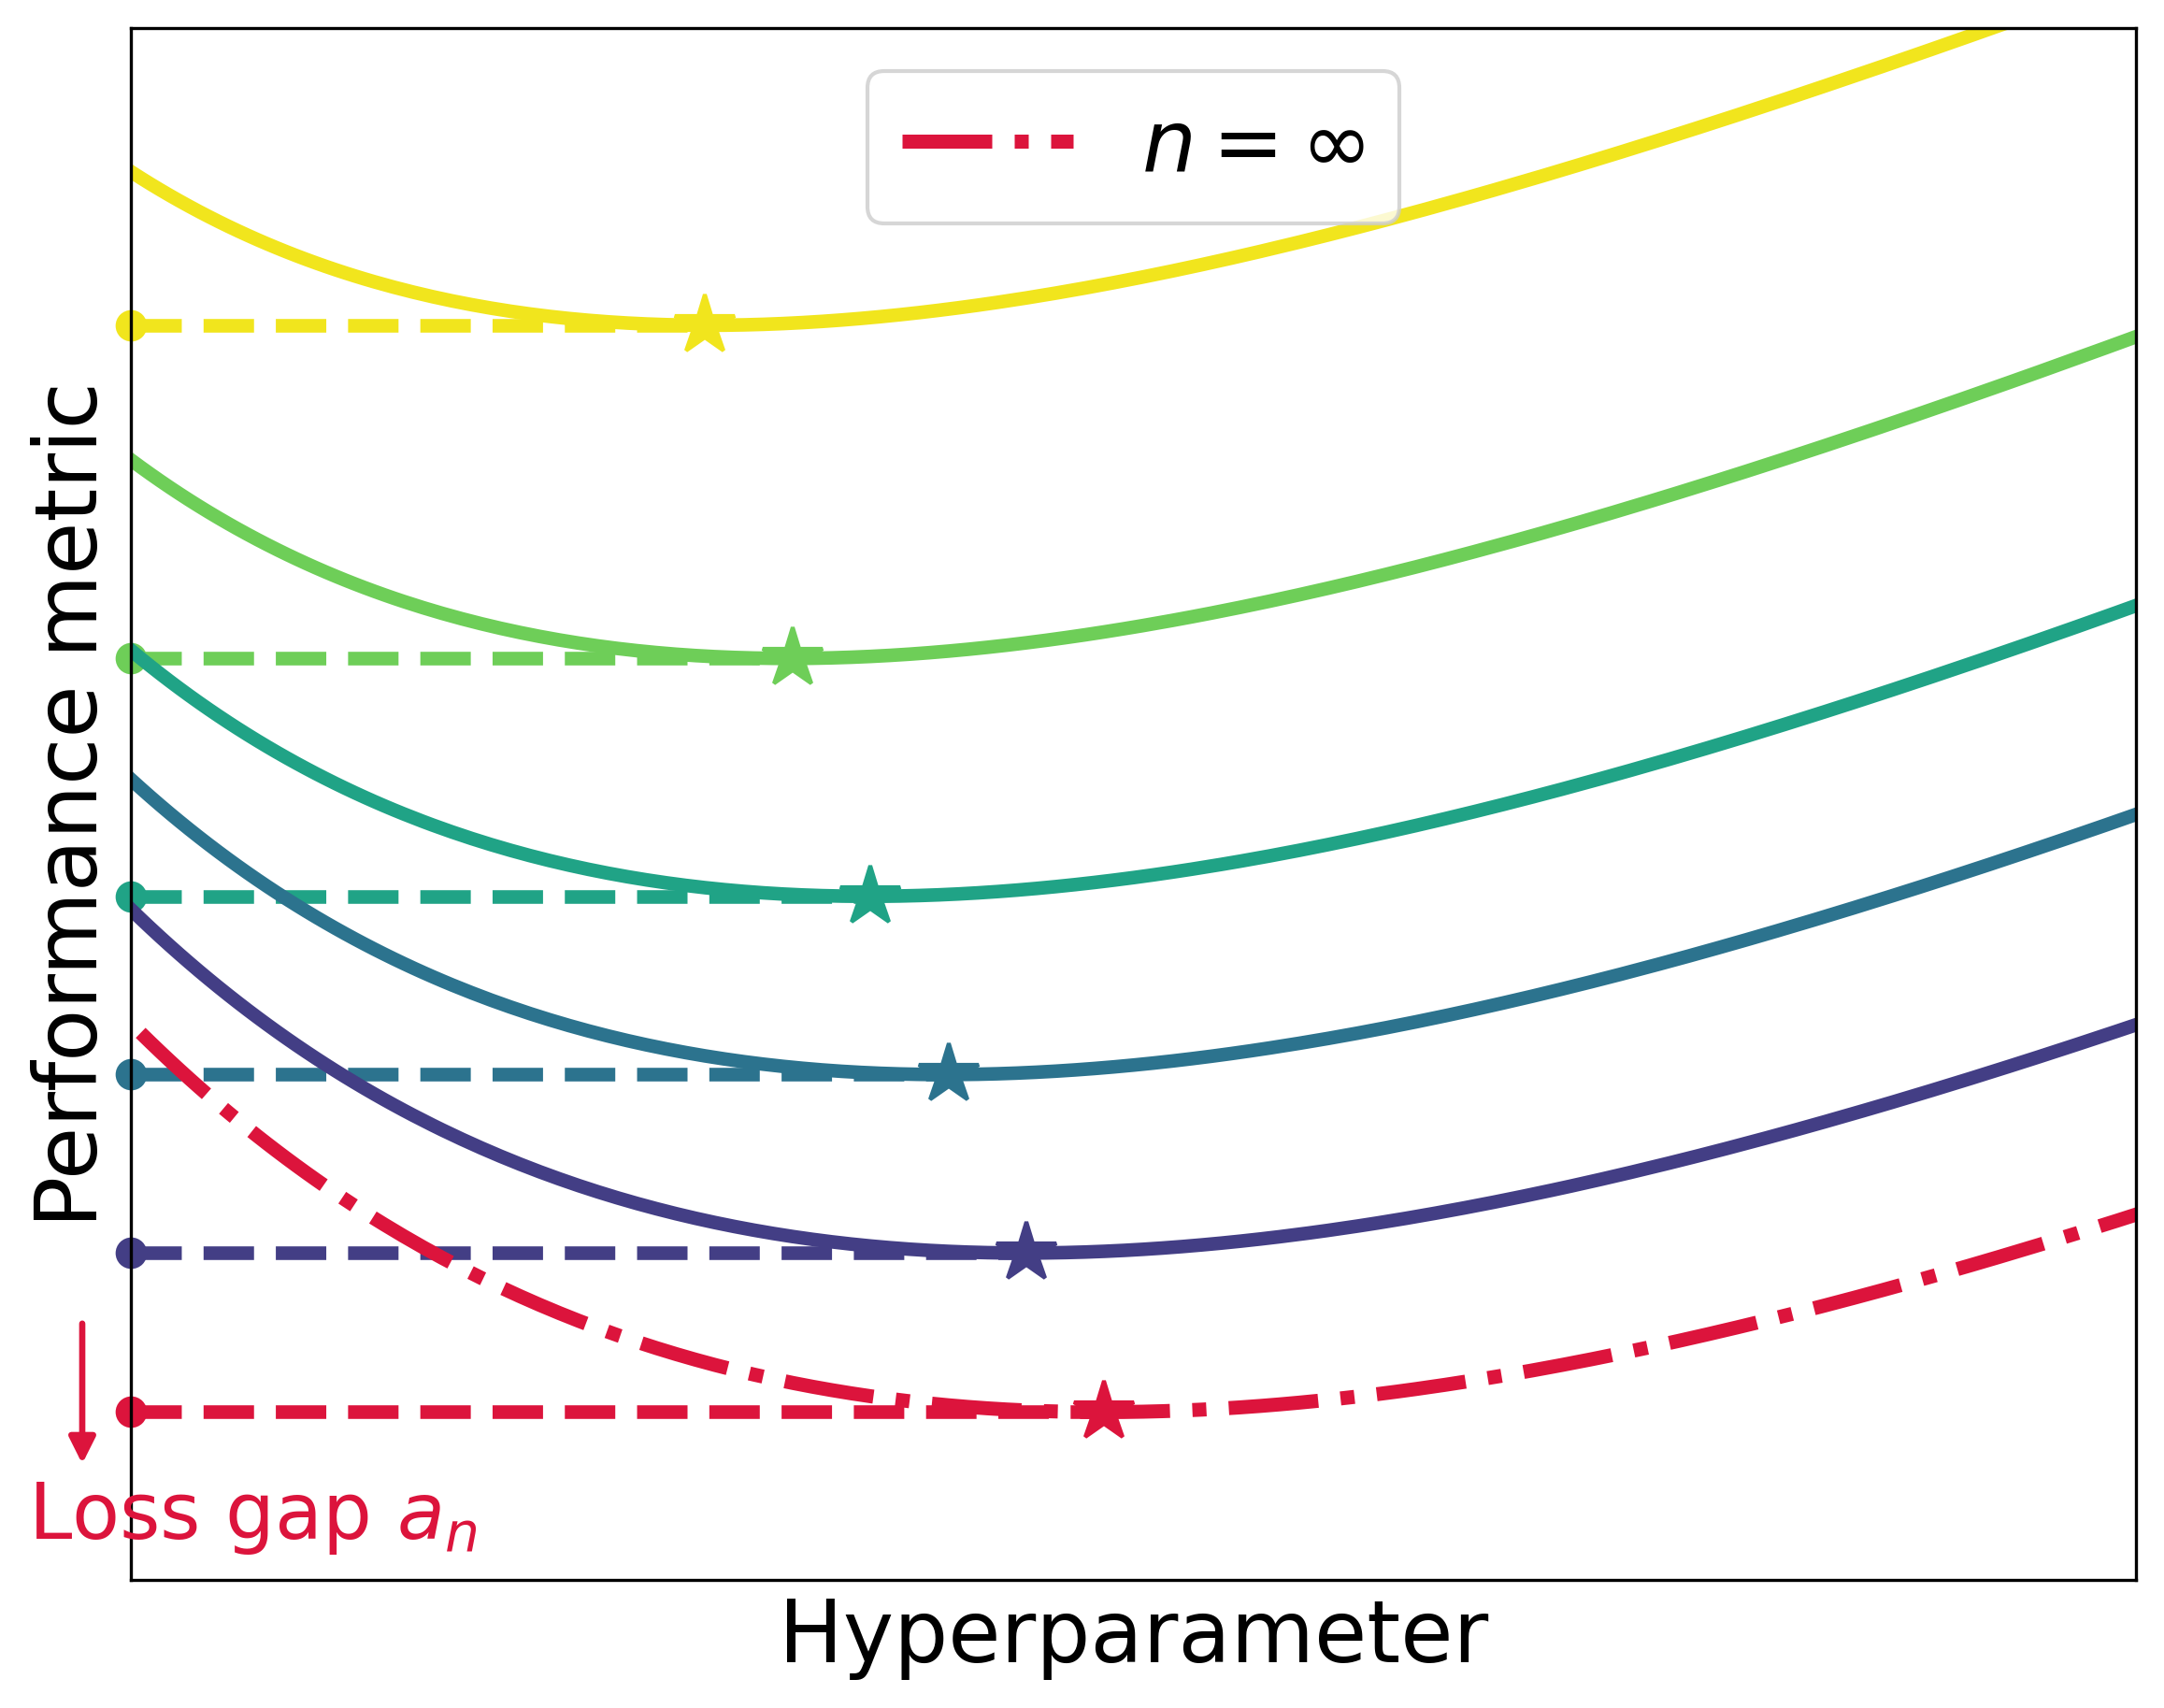
\includegraphics[height=0.73\textwidth]{figures/a_n.png}}  \\ \vspace{-0mm}
\small (a) Loss gap $a_n$.
\end{minipage}%
\begin{minipage}[t]{0.32\linewidth}
\centering 
{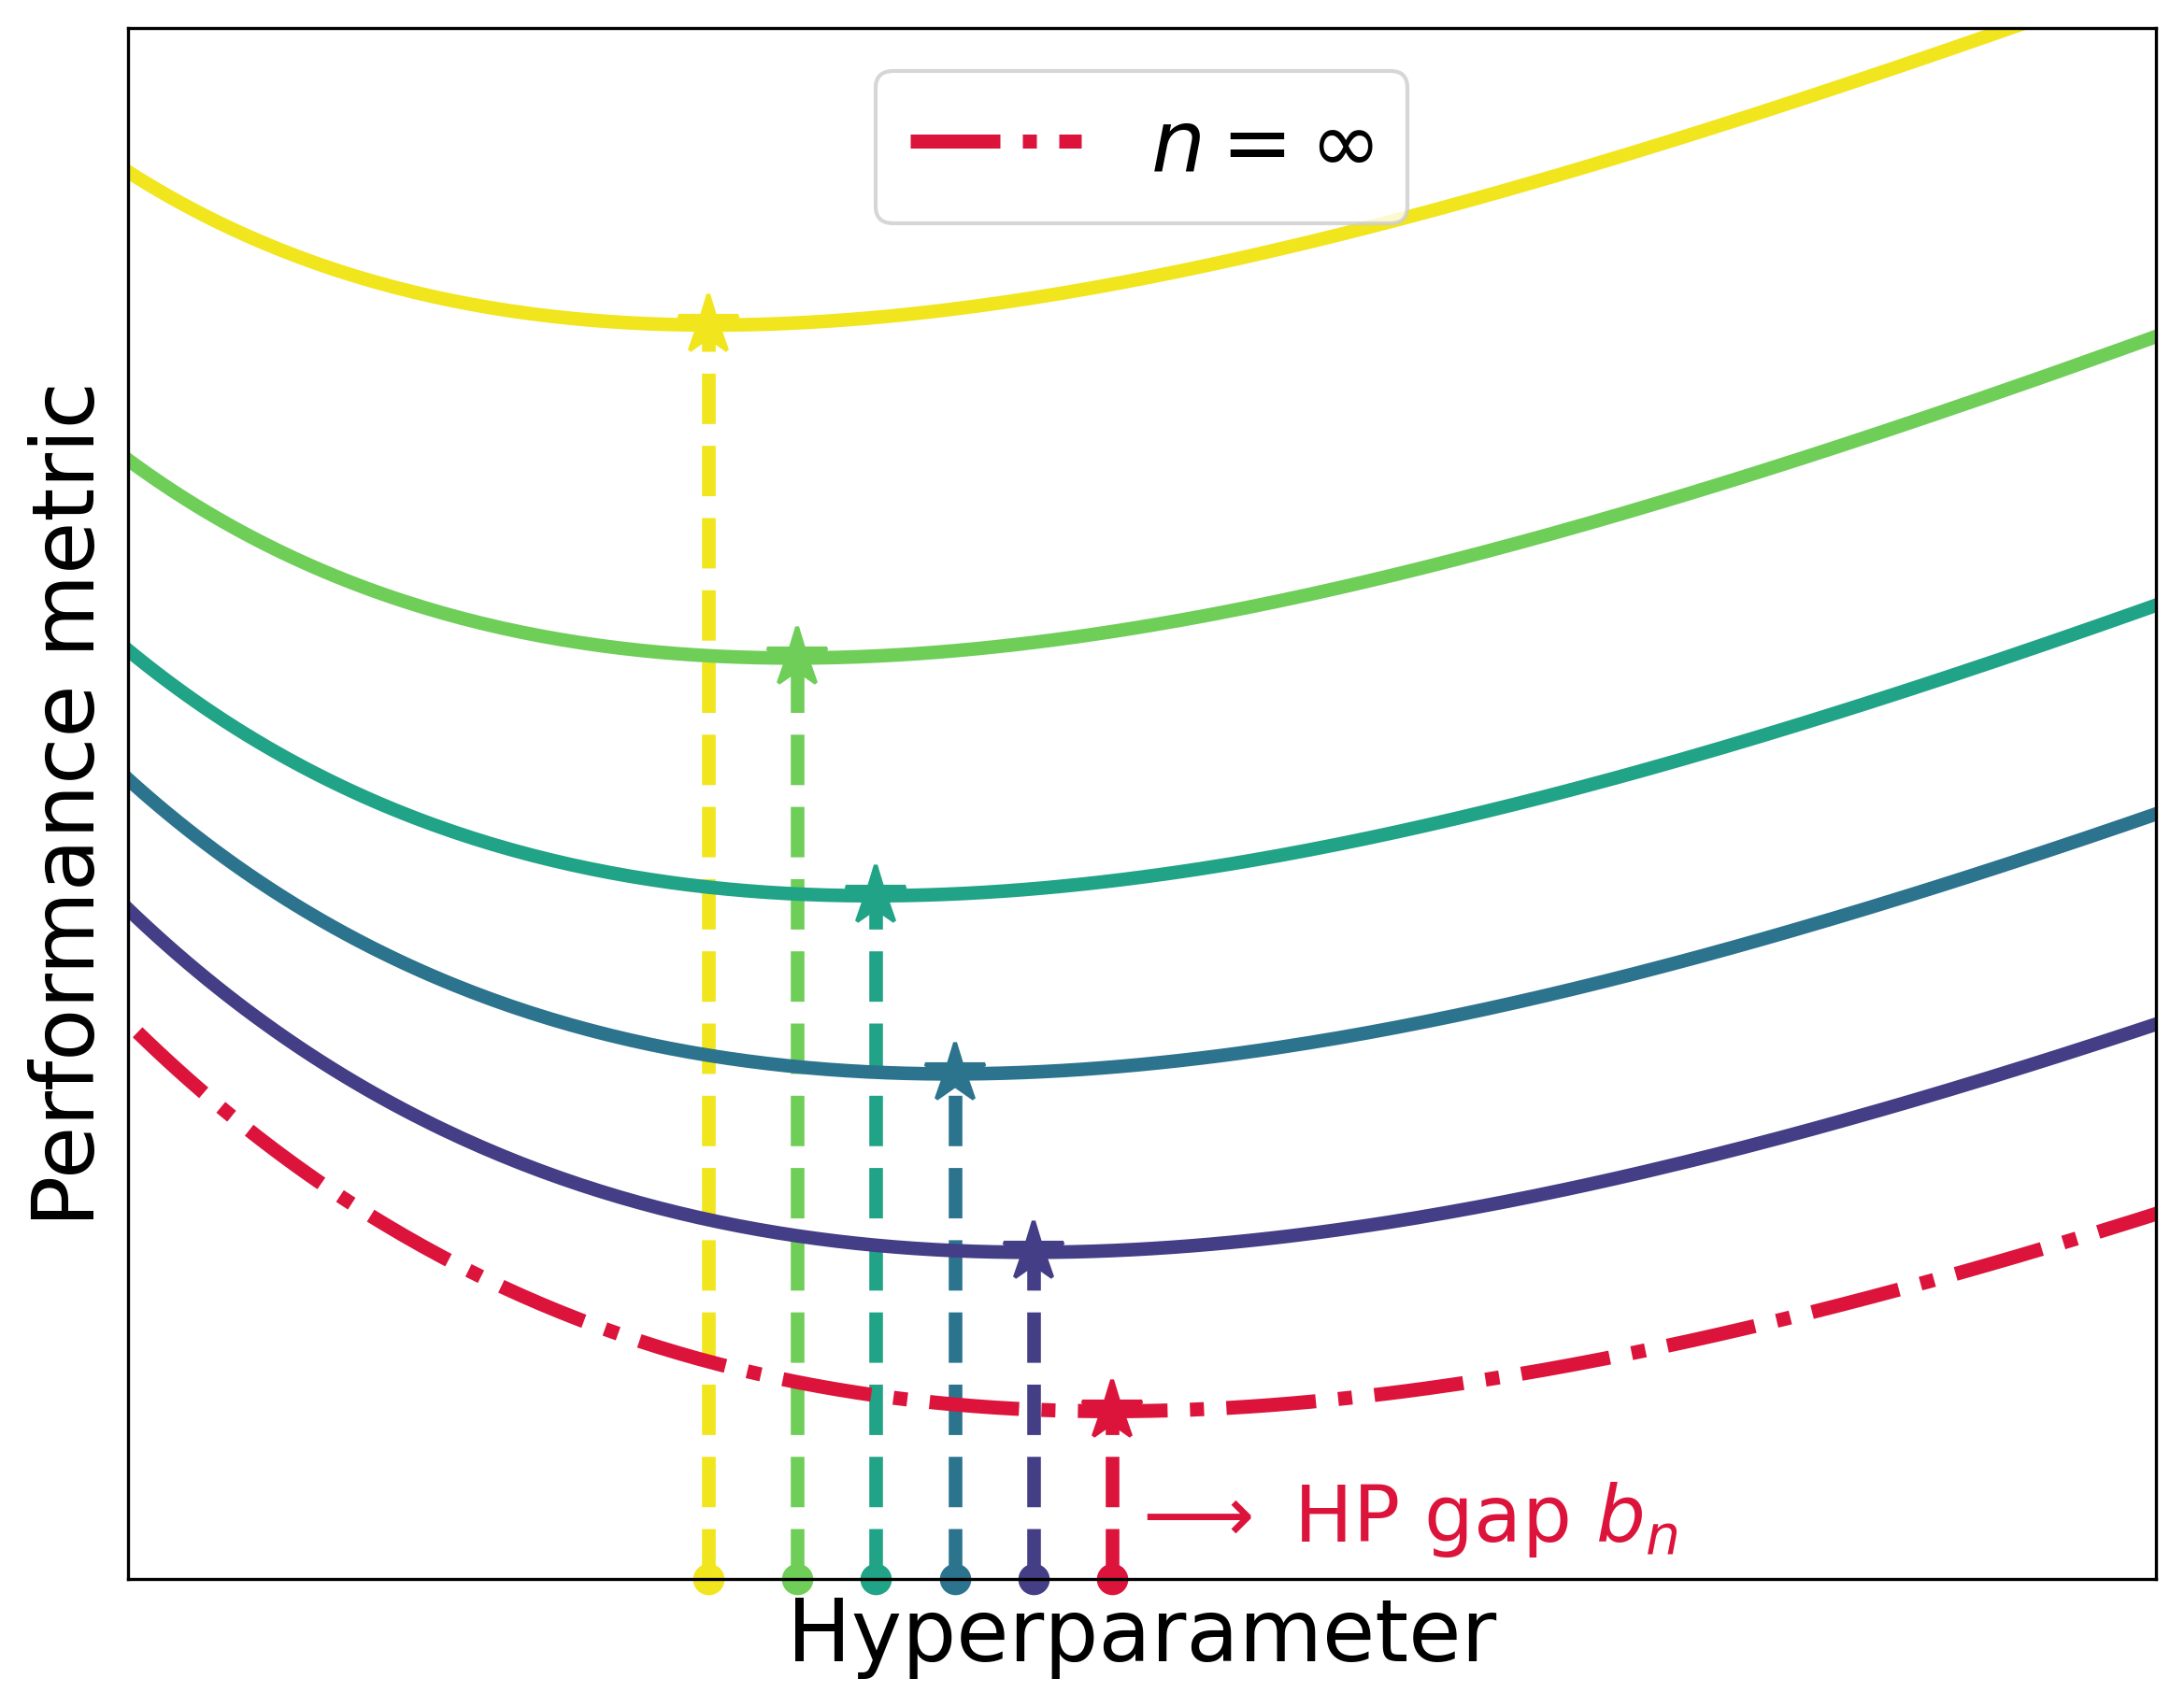
\includegraphics[height=0.73\textwidth]{figures/b_n.png}} \\ \vspace{-0mm}
\small (b) Hyperparameter gap $b_n$. 
\end{minipage}%
\begin{minipage}[t]{0.32\linewidth}
\centering 
{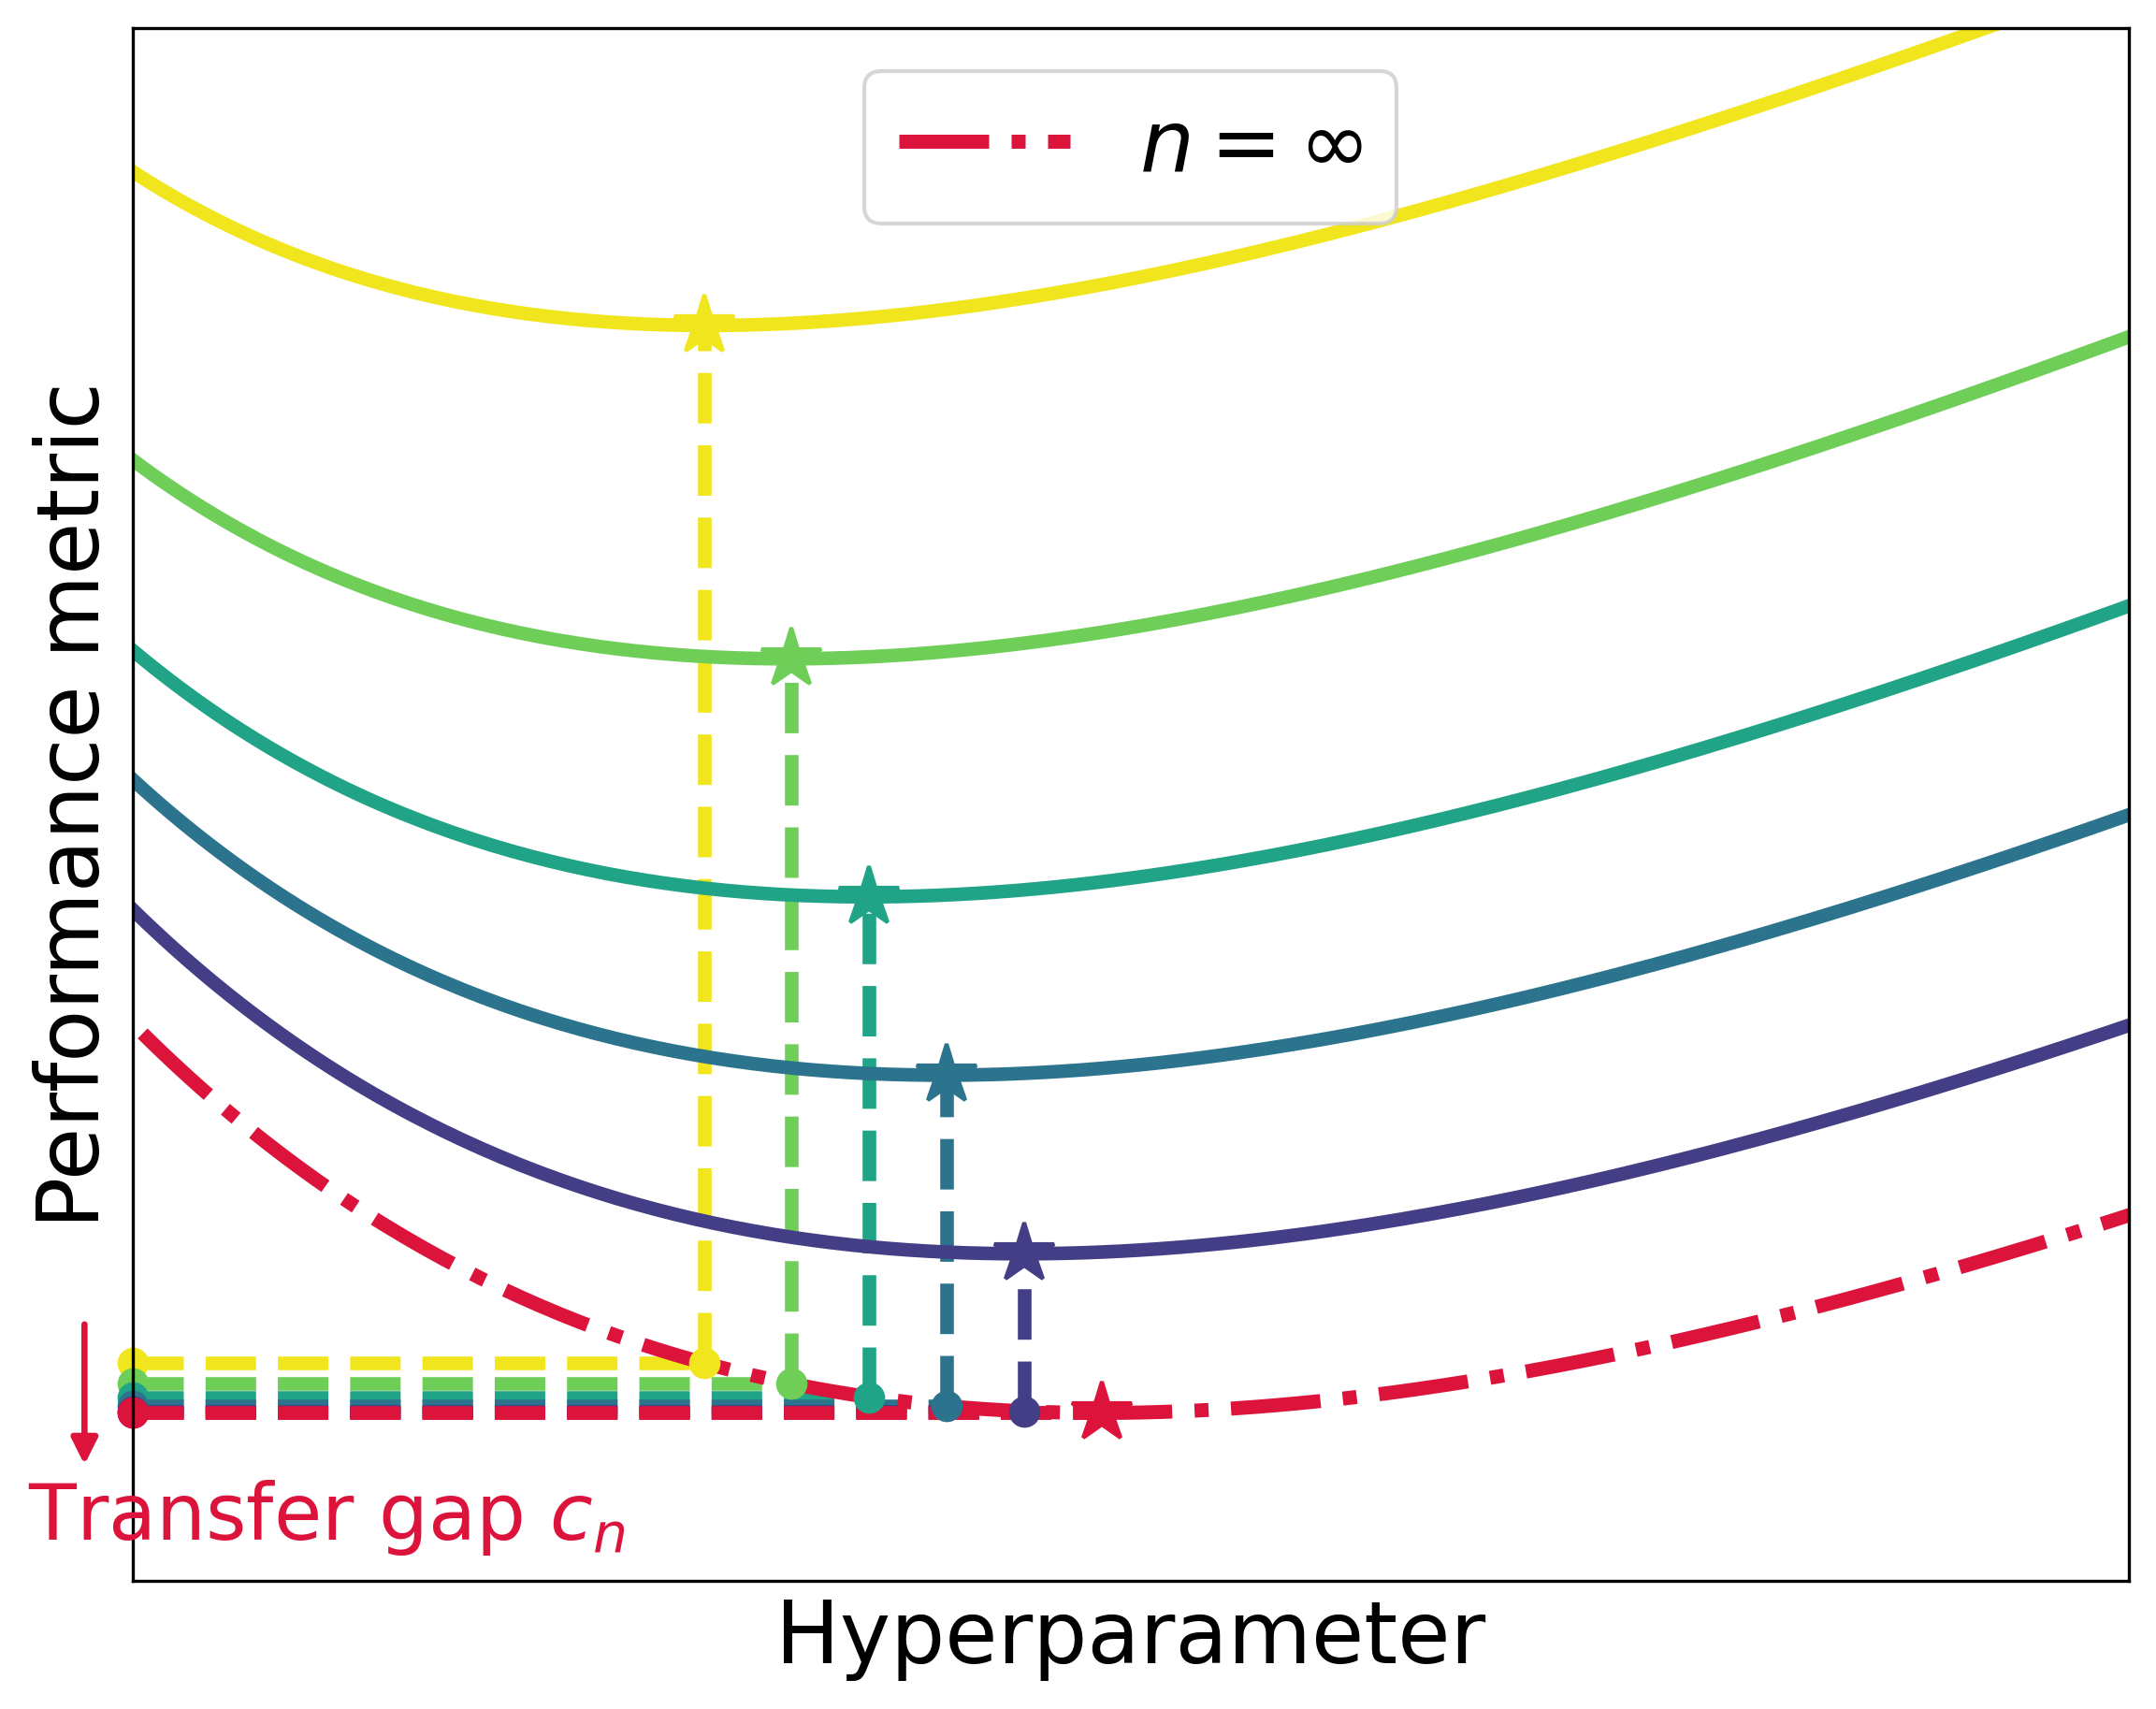
\includegraphics[height=0.73\textwidth]{figures/c_n.png}} \\ \vspace{-0mm}
\small (c) Transfer suboptimality gap $c_n$. 
\end{minipage}%
% \vspace{-1mm} 
\caption{\small Illustration of convergent quantities in Definition~\ref{def:convergent_quantities}; note that $c_n$ captures the efficiency of HP transfer. }  
% \vspace{-1mm}
\label{fig:convergent-quantities} 
\end{figure}  



% \TODO{Reminder on basic asymptotic notation?} 
\paragraph{Fast Transfer.} In the following, in addition to assuming HP transfer holds (Def.\ \ref{def:hp_transfer} in Appendix \ref{app:weak_transfer}) we will make the mild technical assumption that the ``uniform loss gap is locally tight'' which implies that $a_n \sim \supnorm{\phi_n - \phi_\infty}$ (see Def.\ \ref{def:locally_tight} and Lemma \ref{lem:unif_loss_gap} in Appendix \ref{app:asymptotic_rates}). The following proposition uses strong convexity around the optimal infinite-width HP to directly connect the convergence rates of the optimal HP and the evaluation metric (see Appendix~\ref{app:asymptotic_rates}).
\begin{proposition}\label{prop:basic_rate}
     $b_n = O\big(a_n^{1 / 2}\big)$ and $c_n = \Theta(b_n^2) = O(a_n)$.
\end{proposition}
Since HP transfer holds, we have by definition $a_n, b_n, c_n \to 0$ as $n \to \infty$. This being said, \textit{a priori} we may have $b_n = \Theta\big(a_n^{1/2}\big)$ and hence $c_n = \Theta(a_n)$. This would indicate that the transfer suboptimality gap converges at the same rate as the loss gap. In practice however, we tend to observe a much faster rate for $c_n$ relative to $a_n$. We refer to this phenomenon formally as \textit{fast transfer}.
\begin{definition}
We say that HP transfer is fast if $c_n = o(a_n)$ which occurs iff $b_n = o\big(a_n^{1/2}\big)$.
    \label{def:fast-transfer}
\end{definition}
For instance, if $a_n \sim n^{-\alpha}$ and $b_n \sim n^{-\beta}$, then fast transfer occurs if and only if $ \beta > \alpha / 2$. 

\paragraph{Useful Transfer.} It turns out that the notion of fast transfer also coincides with the computational usefulness of HP transfer when performing a grid search. More precisely, consider two HP tuning strategies: \textbf{direct} performs grid search on models of a single width, and \textbf{transfer} performs grid search on models of a smaller width and then trains a final model of larger width using the obtained optimal HPs.  
Suppose we have a compute budget of $\flops$ flops, and the amount of flops needed for a single training run scales with $n^{\compexp}$ for models of width $n$, where $\compexp = 2$ for standard optimization algorithms on standard architectures. 
We say that transfer is \textit{useful} if the transfer strategy yields better performance than the direct strategy for a given compute budget. The following result (formally detailed in Appendix \ref{app:grid_search}) characterizes when this occurs. 

\begin{theorem}[Useful transfer]\label{thm:grid_and_transfer_rate}
Suppose $a_n \sim n^{-\alpha}$ and $b_n \sim n^{-\beta}$. We are given a compute budget of $\flops$ flops, we tune $\numhps$ different HPs, and a single training run at width $n$ costs $n^{\compexp}$ flops. 
\begin{enumerate}[label=(\alph*),leftmargin=*,]
    \item \textbf{Direct tuning.} If we directly conduct grid search on a width-$n$ model, the compute-optimal performance scales as $\flops^{\frac{-2\alpha}{\numhps \alpha + 2 \compexp}}$ and is obtained at width $n^\star \sim \flops^{\frac{2}{\numhps \alpha + 2 \compexp}}$.
    \item \textbf{Transfer.} If we conduct a grid search on a width-$n$ model and then transfer to a large width-$M$ model, the compute-optimal performance scales as $\flops^{\frac{-\alpha}{\compexp}} + \flops^{\frac{-2\beta}{\numhps \beta + \compexp}}$, obtained at widths $n^\star \sim \flops^{\frac{1}{\numhps \beta + \compexp}}$ and $M^\star \sim \flops^{1/\compexp}$. 
\end{enumerate}
Hence transfer is useful if and only if $\beta > \alpha / 2$, i.e., $b_n = o(\sqrt{a_n})$. 
\end{theorem}

Observe that the requirement $\beta>\alpha/2$ is the same condition as \textit{fast transfer} (Definition~\ref{def:fast-transfer}). Consequently, under local strong convexity of $\phi_\infty$ with respect to $\bhp$ (i.e., at infinite width the model performance
meaningfully degrades away from the optimal HP), the naive loss convergence rate already implies that \textit{transfer never underperforms the direct tuning strategy asymptotically} provided that the HPs are parameterized to be $n$-independent. 
While this observation supports the effectiveness of $\mu$-transfer \citep{yang2022tensor}, it does not address the question of when the optimal HPs converge faster than what is implied naively by the loss convergence (i.e., transfer \textit{outperforming} direct tuning). The question turns out to be subtle, and the following subsection presents simple examples where fast transfer may be present or absent. 

\subsection{Examples of Fast and Slow HP Transfer}\label{sec:examples}

Note that the precise scaling of quantities in Definition~\ref{def:convergent_quantities} is infeasible to measure in large-scale scenarios: since the infinite-scale model ($n\to\infty$) is inaccessible, we must resort to power-law fits from finite-$n$ data, which requires a fine grid search of HPs at each scale. Consequently, in this section we present synthetic settings where the convergence rate of $(a_n,b_n,c_n)$ can be either analytically derived or reliably estimated from data. These settings allow us to quantify whether HP transfer offers computational gain. 


\paragraph{Fast HP Transfer: Random Features Regression.} First we consider tuning the ridge penalty $\lambda$ in a high-dimensional random features (RF) model with nonlinearity $\sigma$, where the target function is a single-index model with link function $\sigma_*$ on isotropic Gaussian input in $\R^d$. We aim to select the optimal regularization parameter $\lambda\in\R$ that minimizes the prediction risk $\mathcal{R}(f) = \E_{\bx} [(y - f(\bx))^2]$. 

In the proportional limit where the number of training data $N$, dimension of input features $d$, and model width $n$ all diverge $N,d,n\to\infty, N/d\to\psi_1, n/d\to\psi_2$ where $\psi_1,\psi_2\in (0,\infty)$, \cite{mei2022generalization,gerace2020generalisation} derived precise asymptotics of prediction risk under standard assumptions (see Assumption~\ref{assumption:RF}). In this model, the number of trainable parameters is controlled by the ratio $\psi_2=n/d$, and the infinite-width model is obtained by sending $\psi_2\to\infty$. The following proposition quantifies the convergence of prediction risk and hyperparameter as a function of $\psi_2$. 

\begin{theorem}\label{thm:RF-rate}
Define $\lambda^*(\psi_2) := \argmin_{\lambda\in\R} \cR_{\psi_2}(\lambda)$, where $\cR_{\psi_2}(\lambda)$ is the asymptotic prediction risk of the RF model with width $n/d=\psi_2$ and ridge penalty $\lambda$. Then under Assumption~\ref{assumption:RF}, we have
\begin{itemize}[leftmargin=*]
    \item \textbf{Loss gap:} $\abs{\cR_{\psi_2}(\lambda^*(\psi_2)) - \cR_{\infty}(\lambda^*(\infty))} = \Theta(\psi_2^{-1})$. 
    \item \textbf{Hyperparameter gap:} $\abs{\lambda^*(\psi_2) - \lambda^*(\infty)} = O(\psi_2^{-1})$. 
    \item \textbf{Suboptimality gap:} $\abs{\cR_\infty(\lambda^*(\psi_2)) - \cR_\infty(\lambda^*(\infty))} = O(\psi_2^{-2})$. 
\end{itemize}
\end{theorem}
This theorem states that both the loss gap $a_n$ and the HP gap $b_n$ scale as $d/n=\psi_2^{-1}$, whereas the transfer suboptimality gap scales as $c_n\sim \psi_2^{-2} \ll a_n$. We conclude that the ridge regularization parameter $\lambda$ exhibits fast transfer per Definition~\ref{def:fast-transfer}. Consequently, Theorem~\ref{thm:grid_and_transfer_rate} implies that tuning the ridge penalty on a small (narrower) RF model and then transfer is more compute-efficient than directly tuning the large-width model. To our knowledge, this gives the first concrete setting where the HP transfer strategy in \cite{yang2023depth} provably offers a computational advantage.   

Figure~\ref{fig:RFF-risk} presents the prediction risk of the RF ridge estimator across varying widths $n/d=\psi_2$. We set $\sigma=\mathrm{tanh}, \sigma_*=\mathrm{ReLU}, \psi_1=4, \sigma_{\varepsilon}=1/4$. The analytical curves are obtained by solving the coupled Stieltjes transforms \eqref{eq:stieltjes1} and \eqref{eq:stieltjes2}. 
Figure~\ref{fig:RFF-scaling} confirms the scaling of $a_n, b_n, c_n$ in Theorem~\ref{thm:RF-rate}.
 
\begin{figure}[t]
\vspace{-2mm} 
\centering
\begin{subfigure}[t]{0.49\linewidth}
\centering
{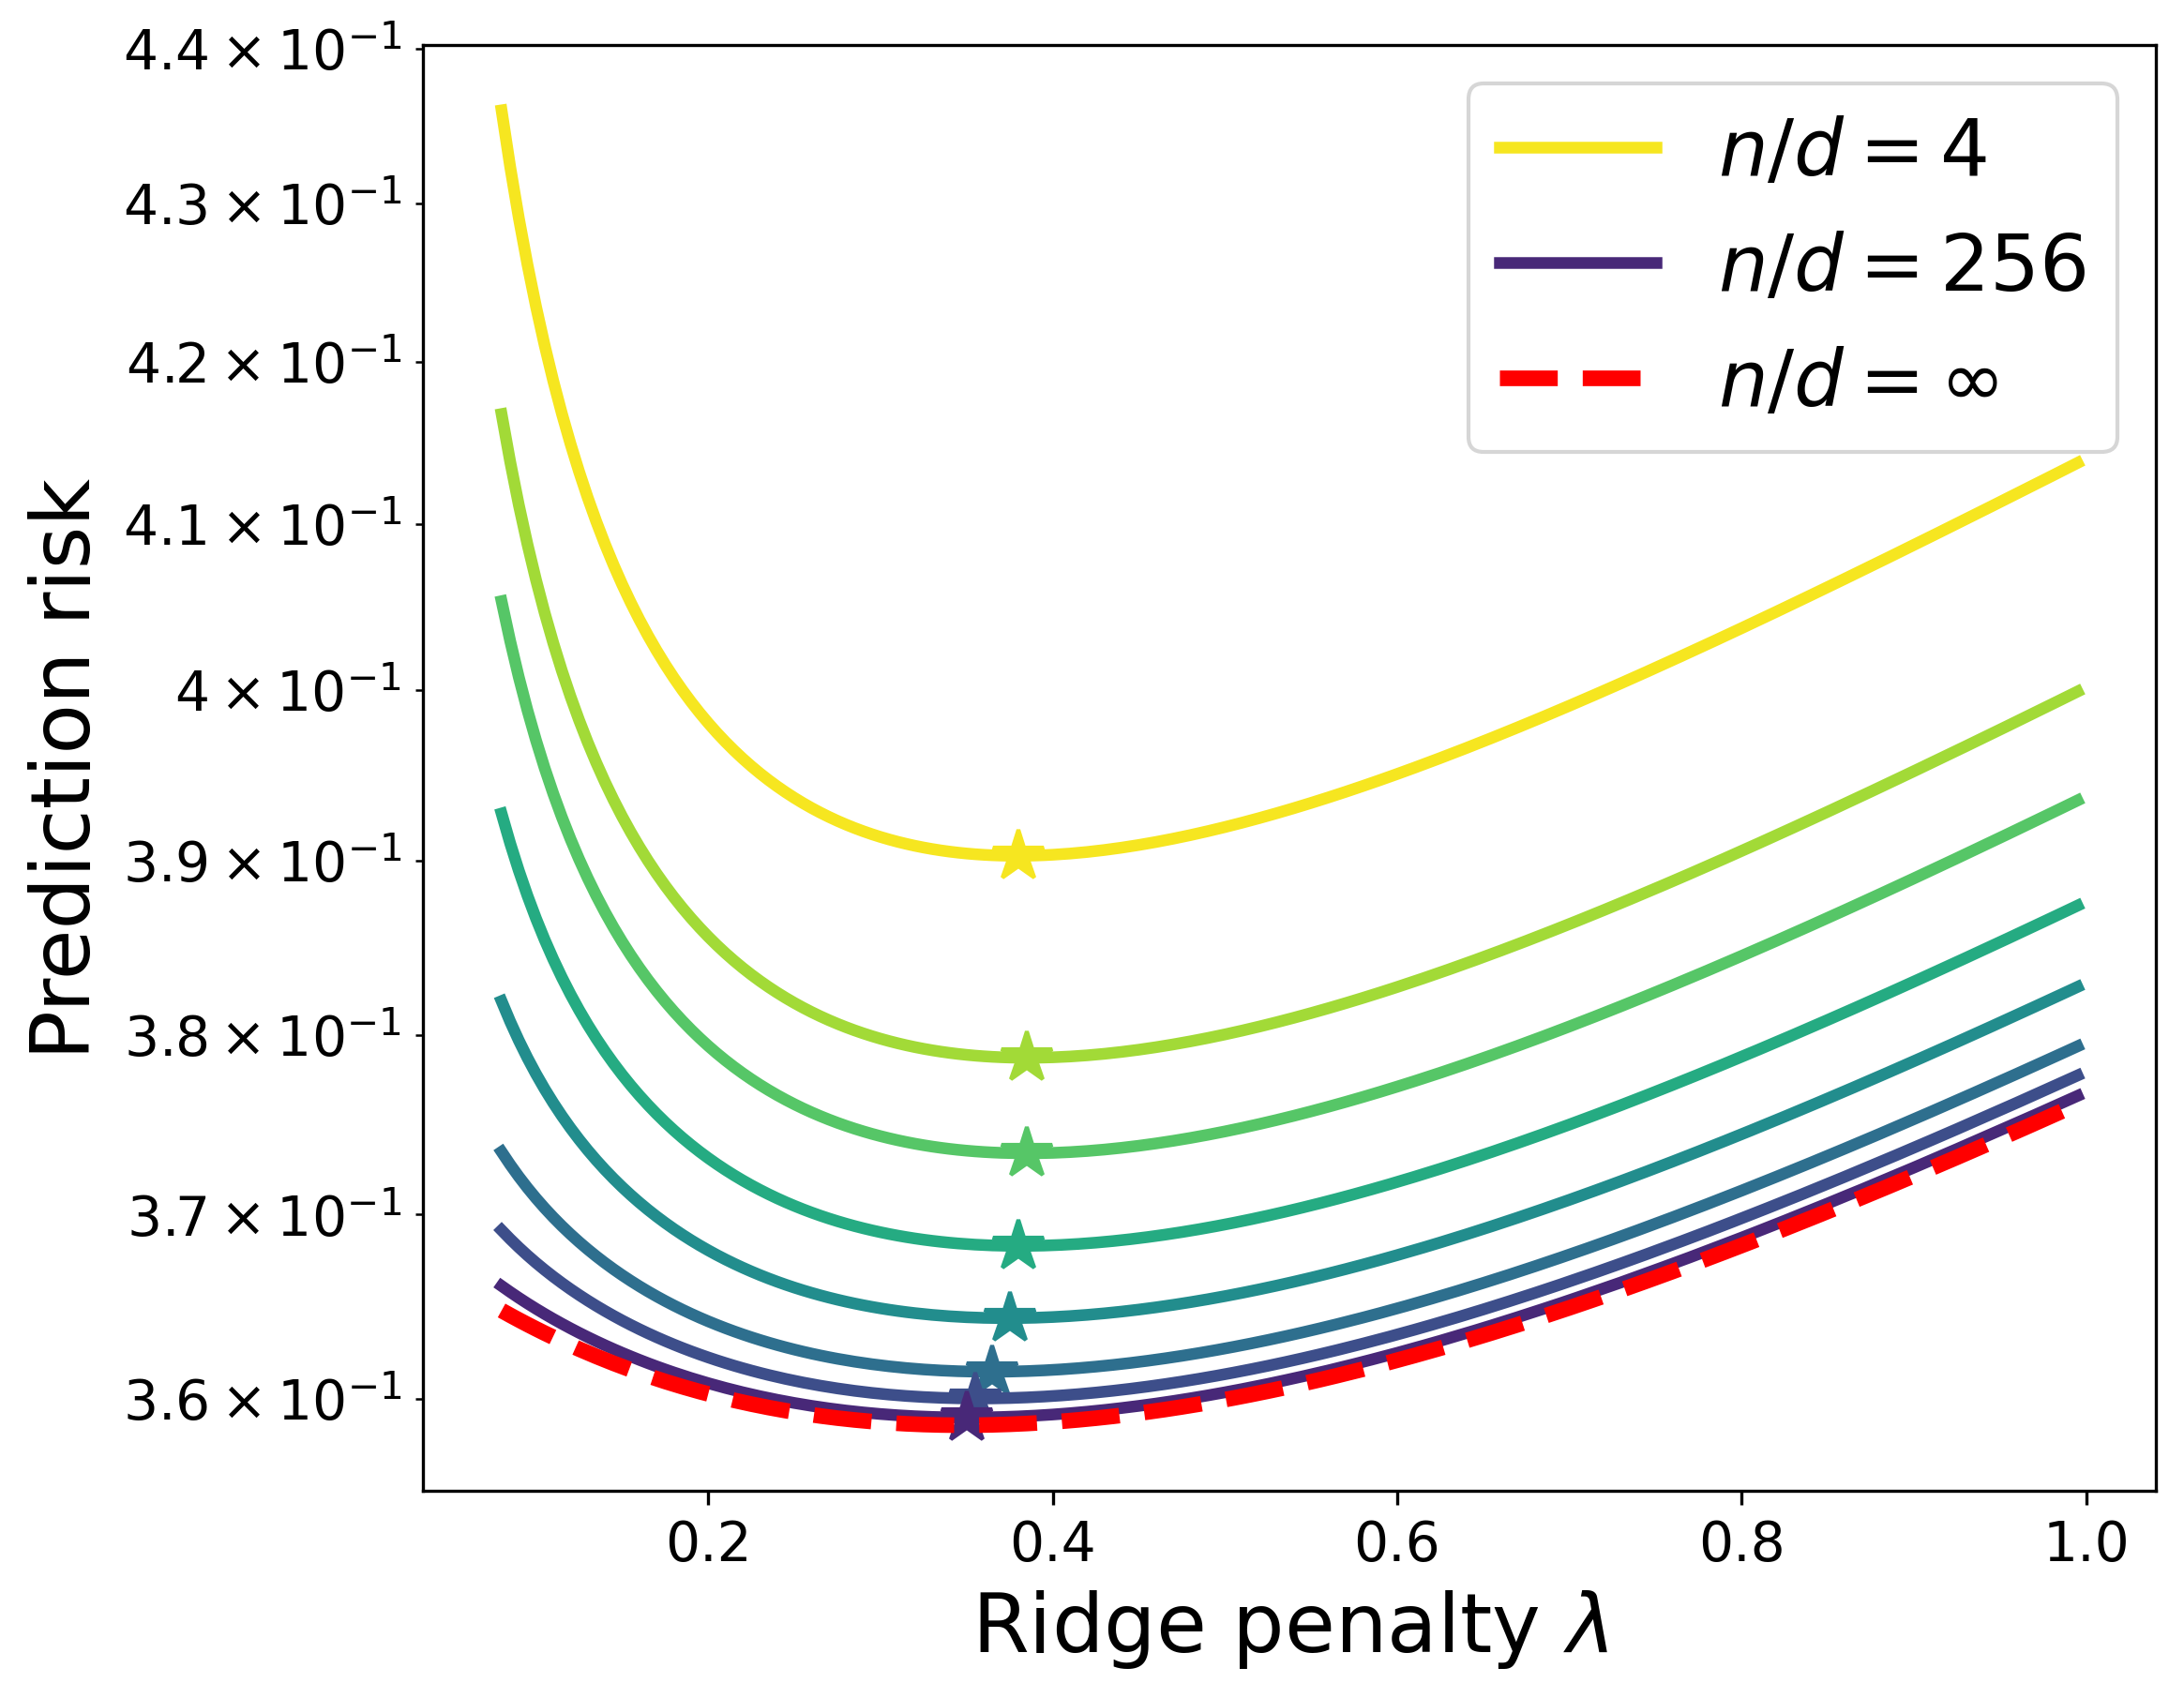
\includegraphics[height=0.69\textwidth]{figures/RFF_loss_new.png}} 
\vspace{-1mm}
\caption{Prediction risk vs.~ridge penalty.}
\label{fig:RFF-risk}
\end{subfigure}%
\begin{subfigure}[t]{0.49\linewidth}
\centering 
{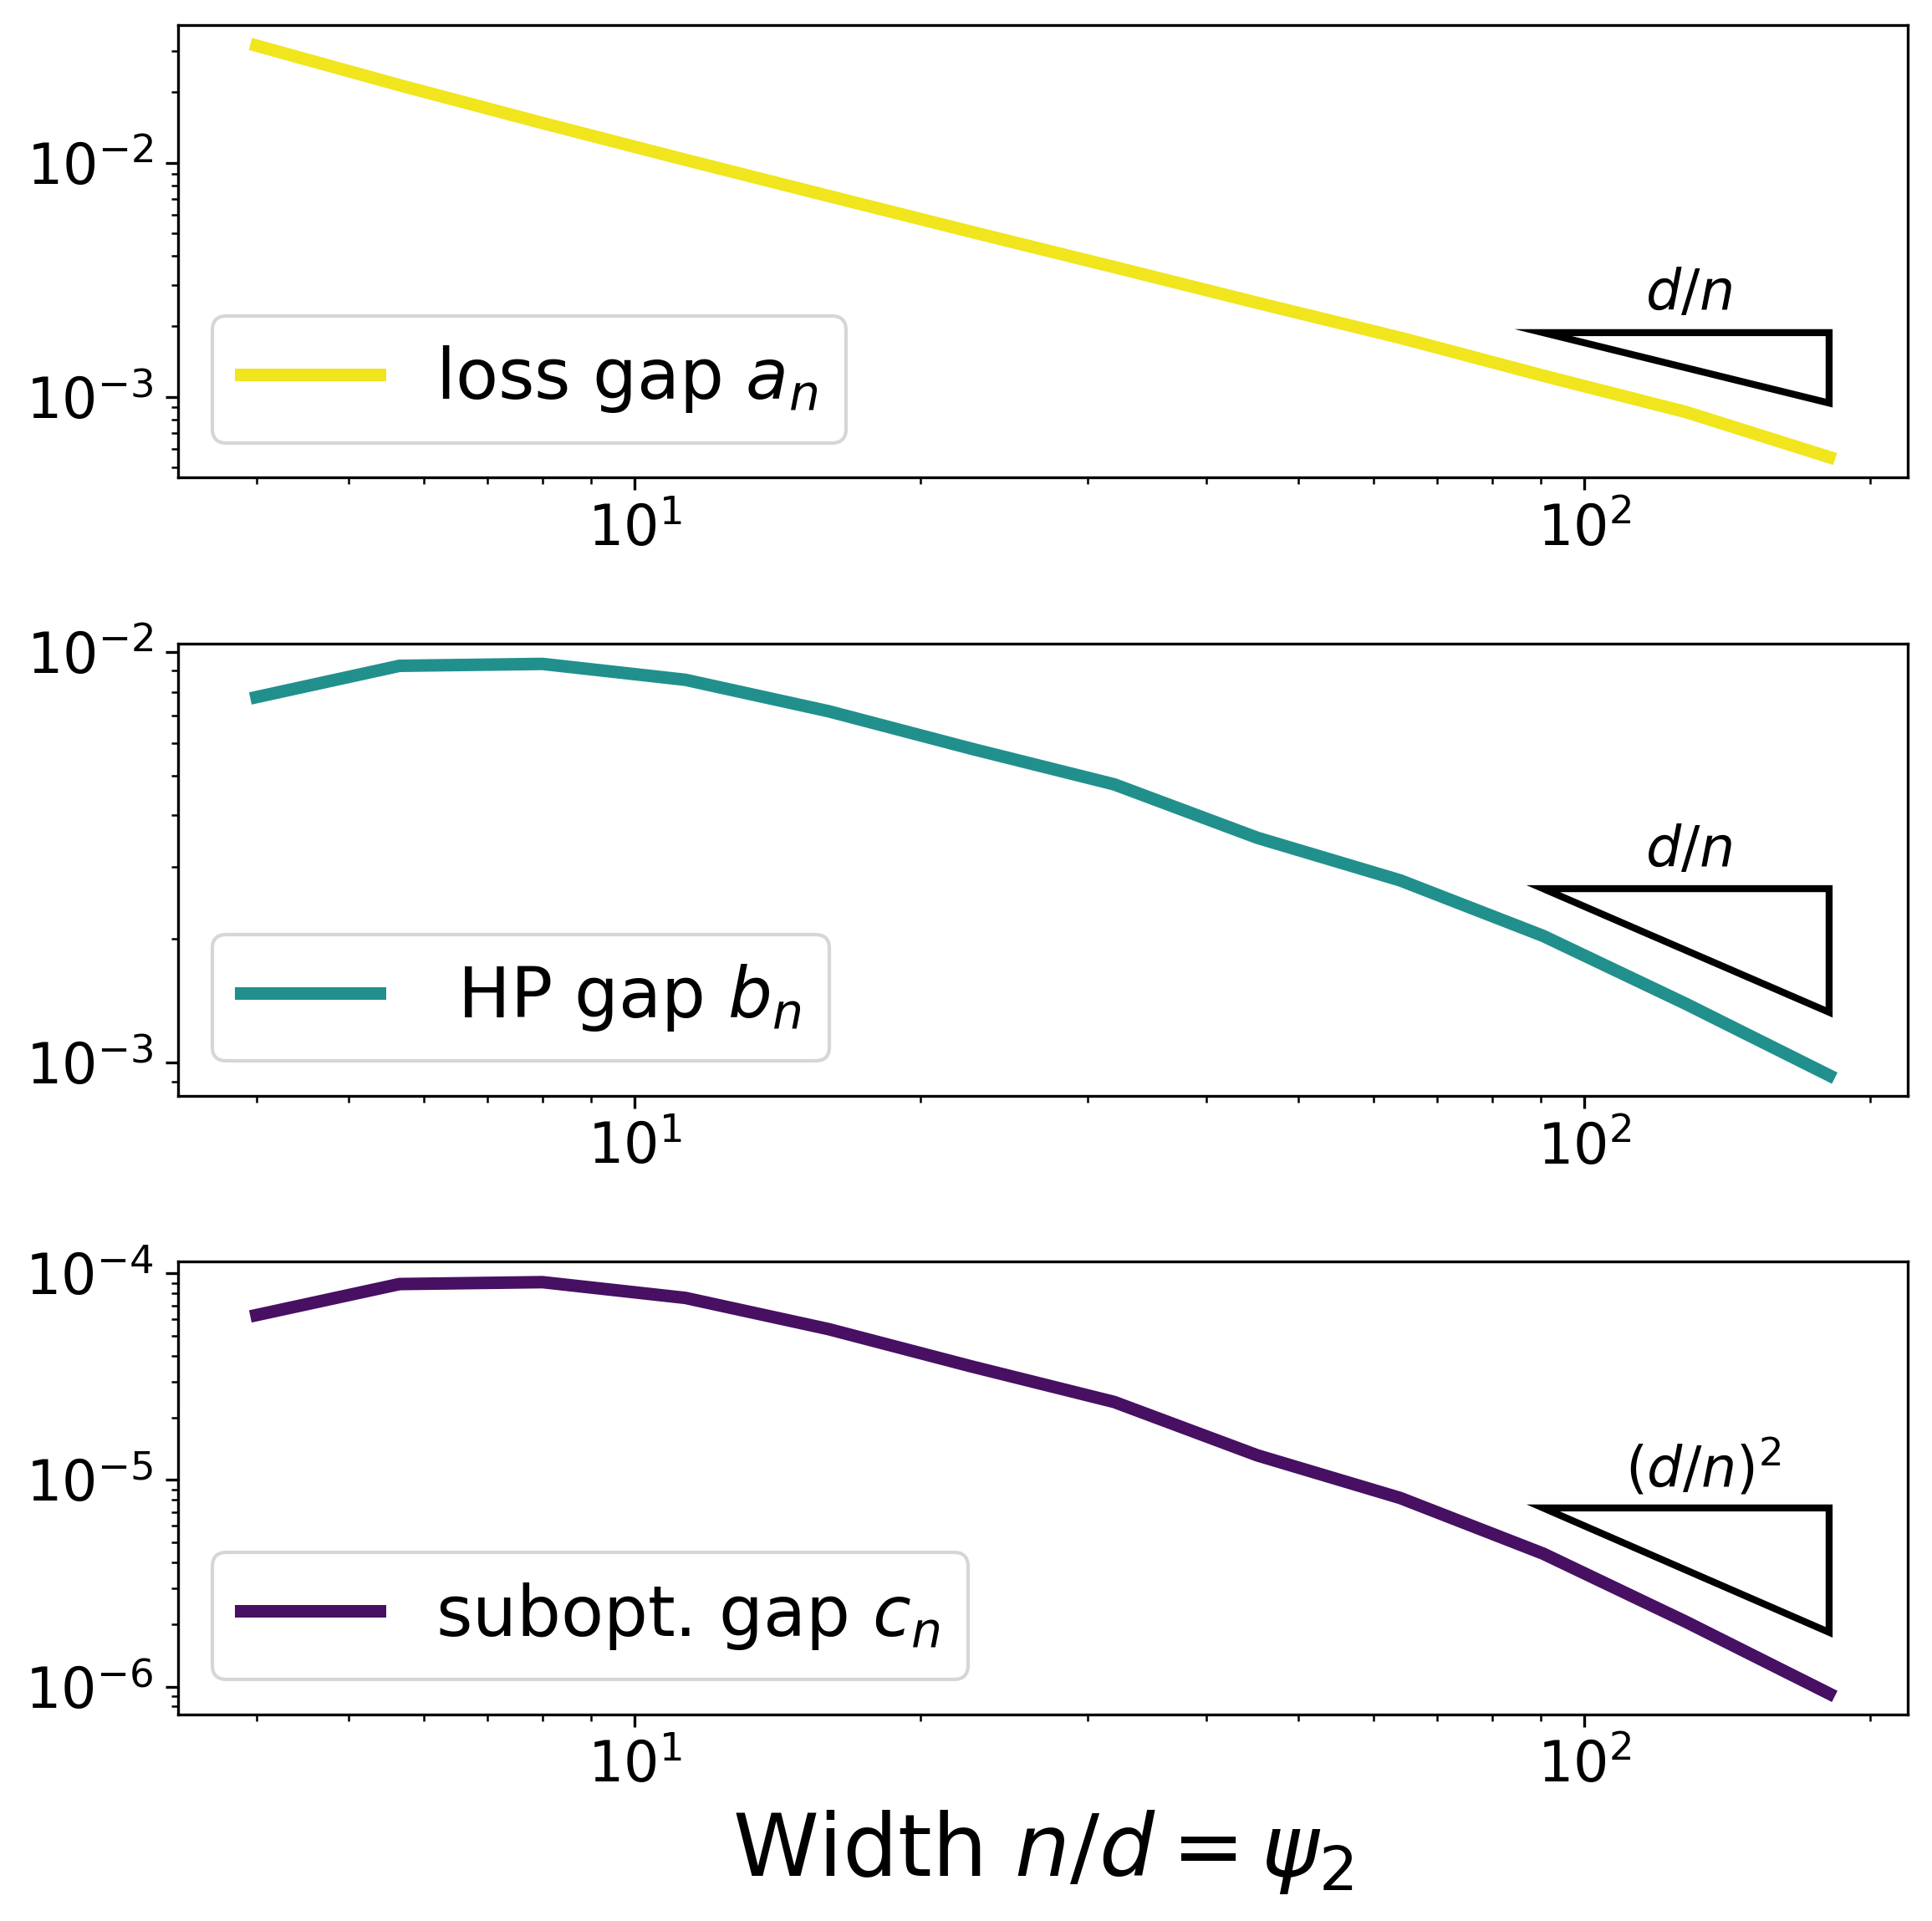
\includegraphics[height=0.69\textwidth]{figures/RFF_rate.png}} 
\vspace{-1mm}
\caption{\small Scaling of optimal loss and ridge penalty.} 
\label{fig:RFF-scaling}
\end{subfigure}%
% \vspace{-1mm} 
\caption{\small Optimal ridge penalty (generalization error) for RF regression to learn a single-index model.}  
\vspace{-0.5mm}
\label{fig:RFF} 
\end{figure}  

\begin{figure}[b]
\vspace{-3mm} 
\centering
\begin{subfigure}[t]{0.49\linewidth}
\centering
{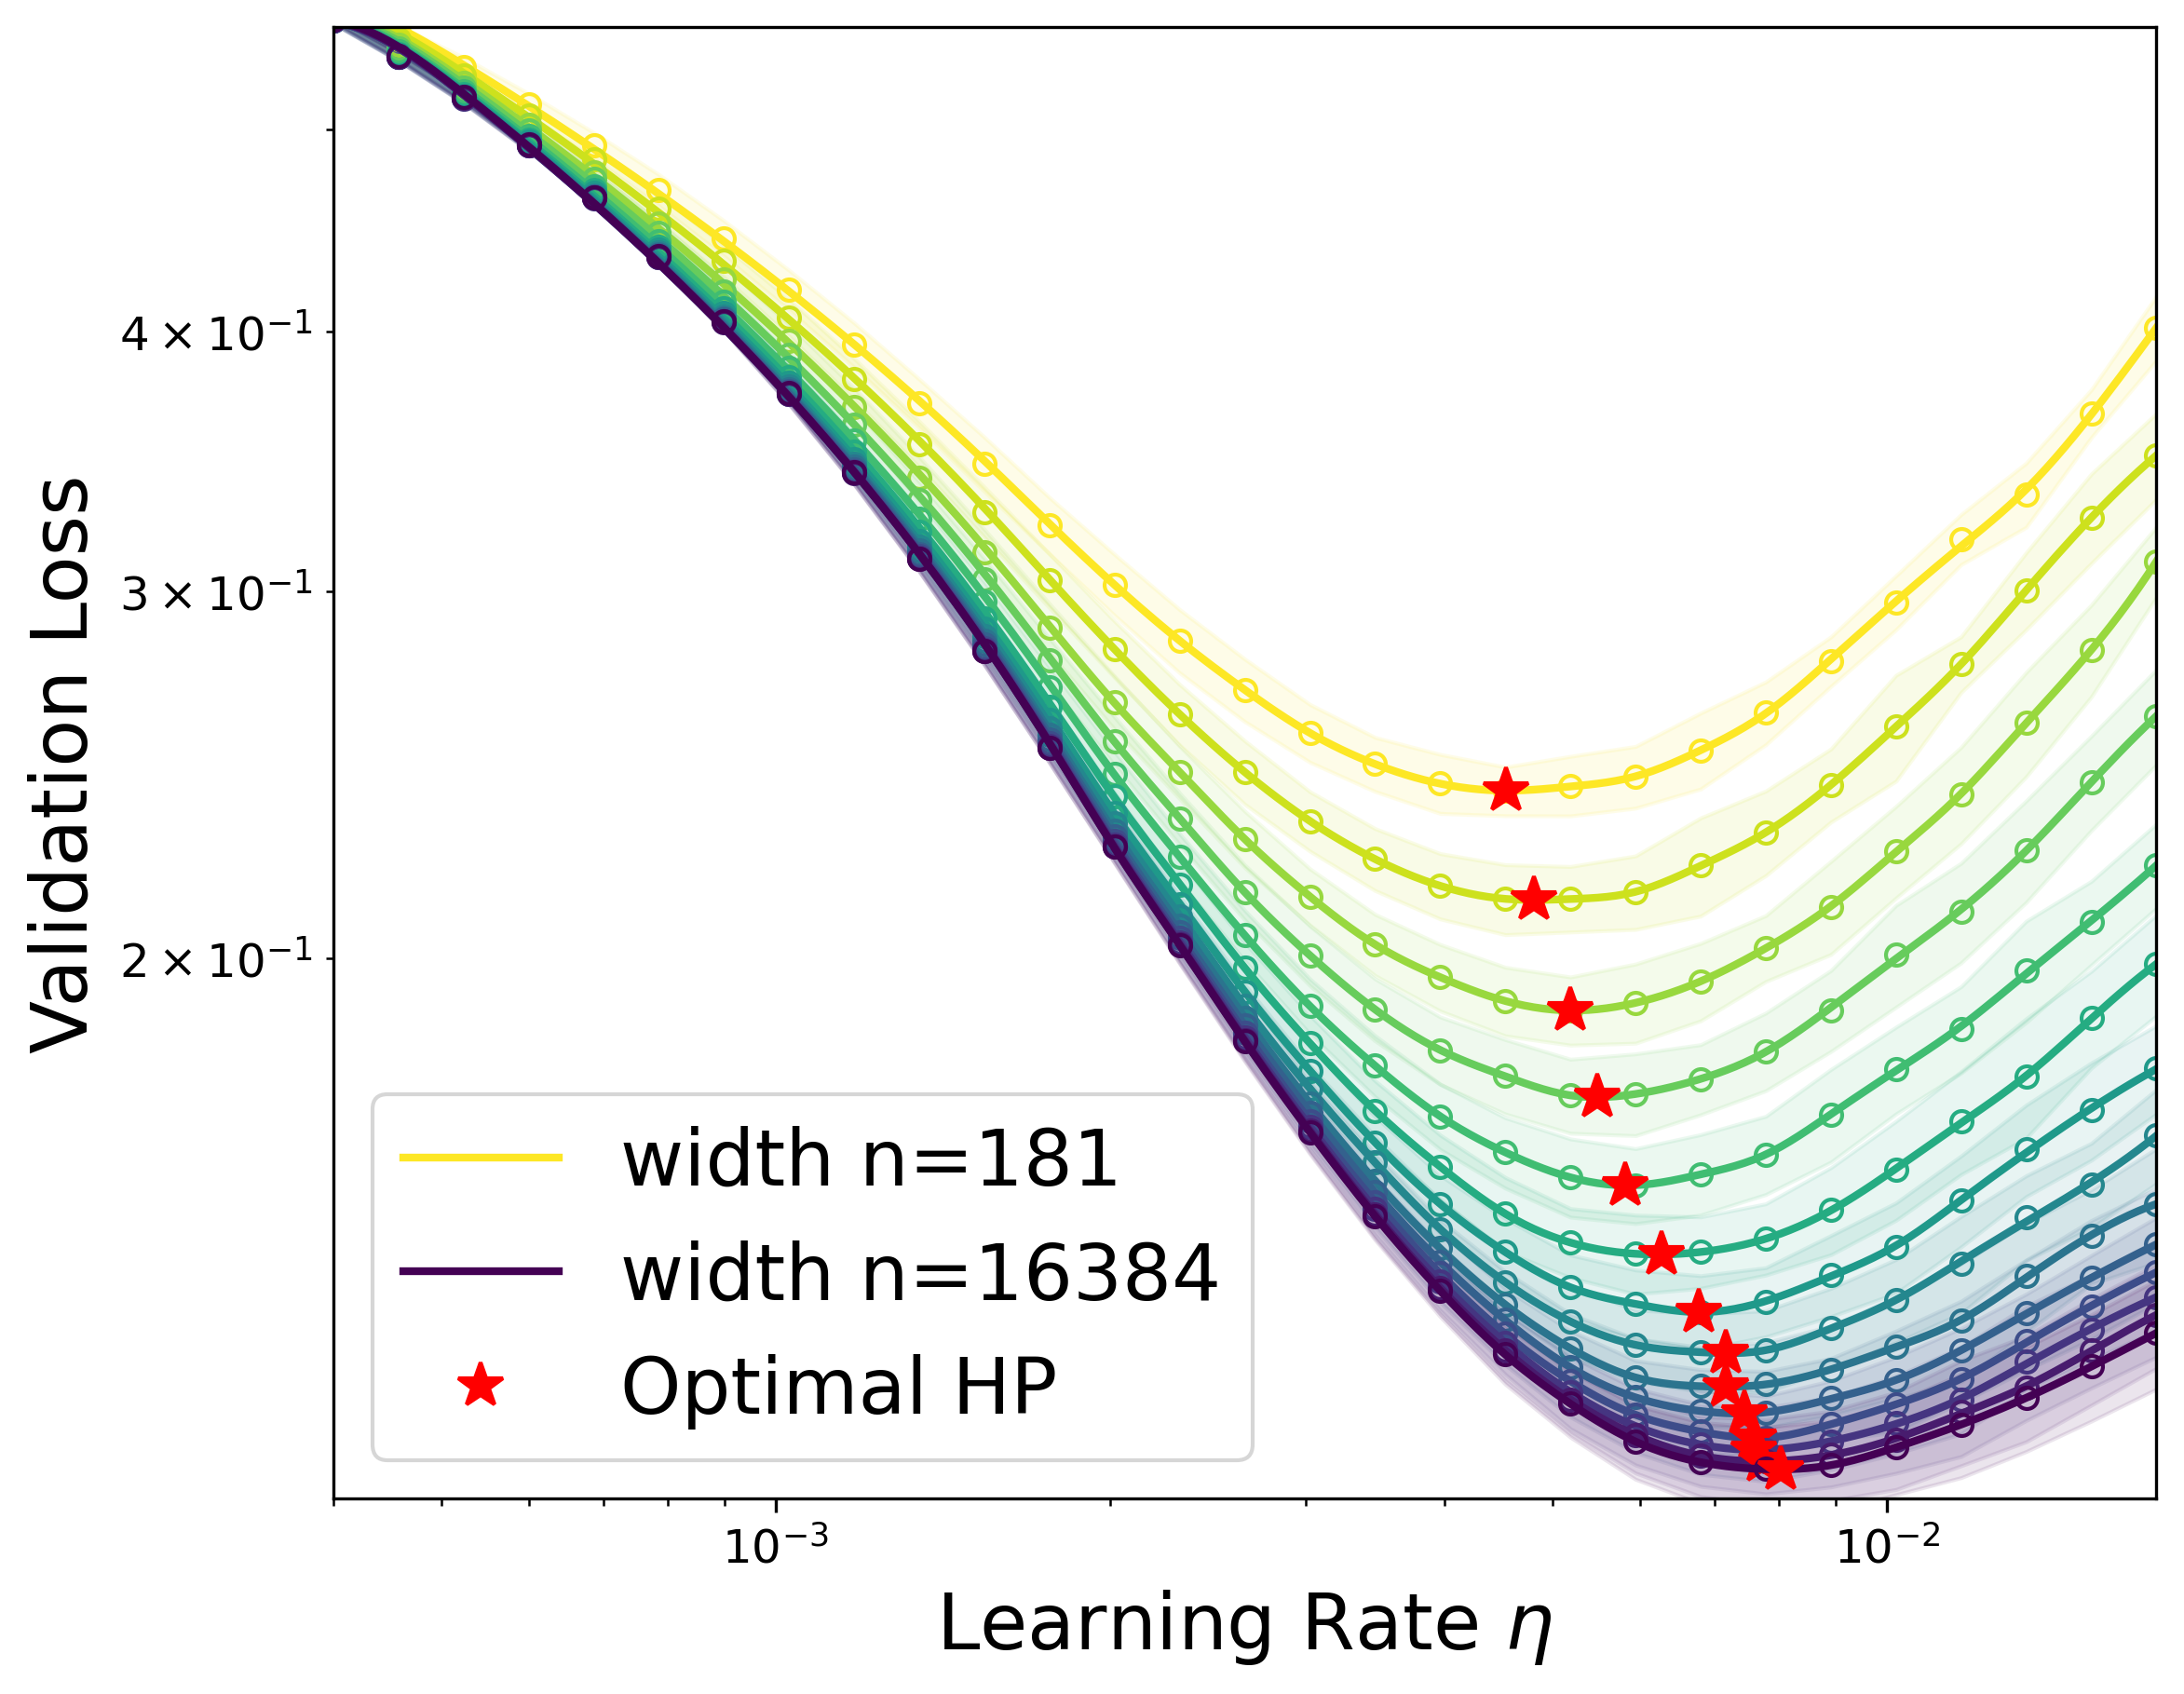
\includegraphics[height=0.65\textwidth]{figures/two_layer_ReLU_loss.png}}  \vspace{-1mm}
\caption{\small Validation loss vs.~learning rate.}
\label{fig:two-layer-ReLU-loss}
\end{subfigure}%
\begin{subfigure}[t]{0.49\linewidth}
\centering 
{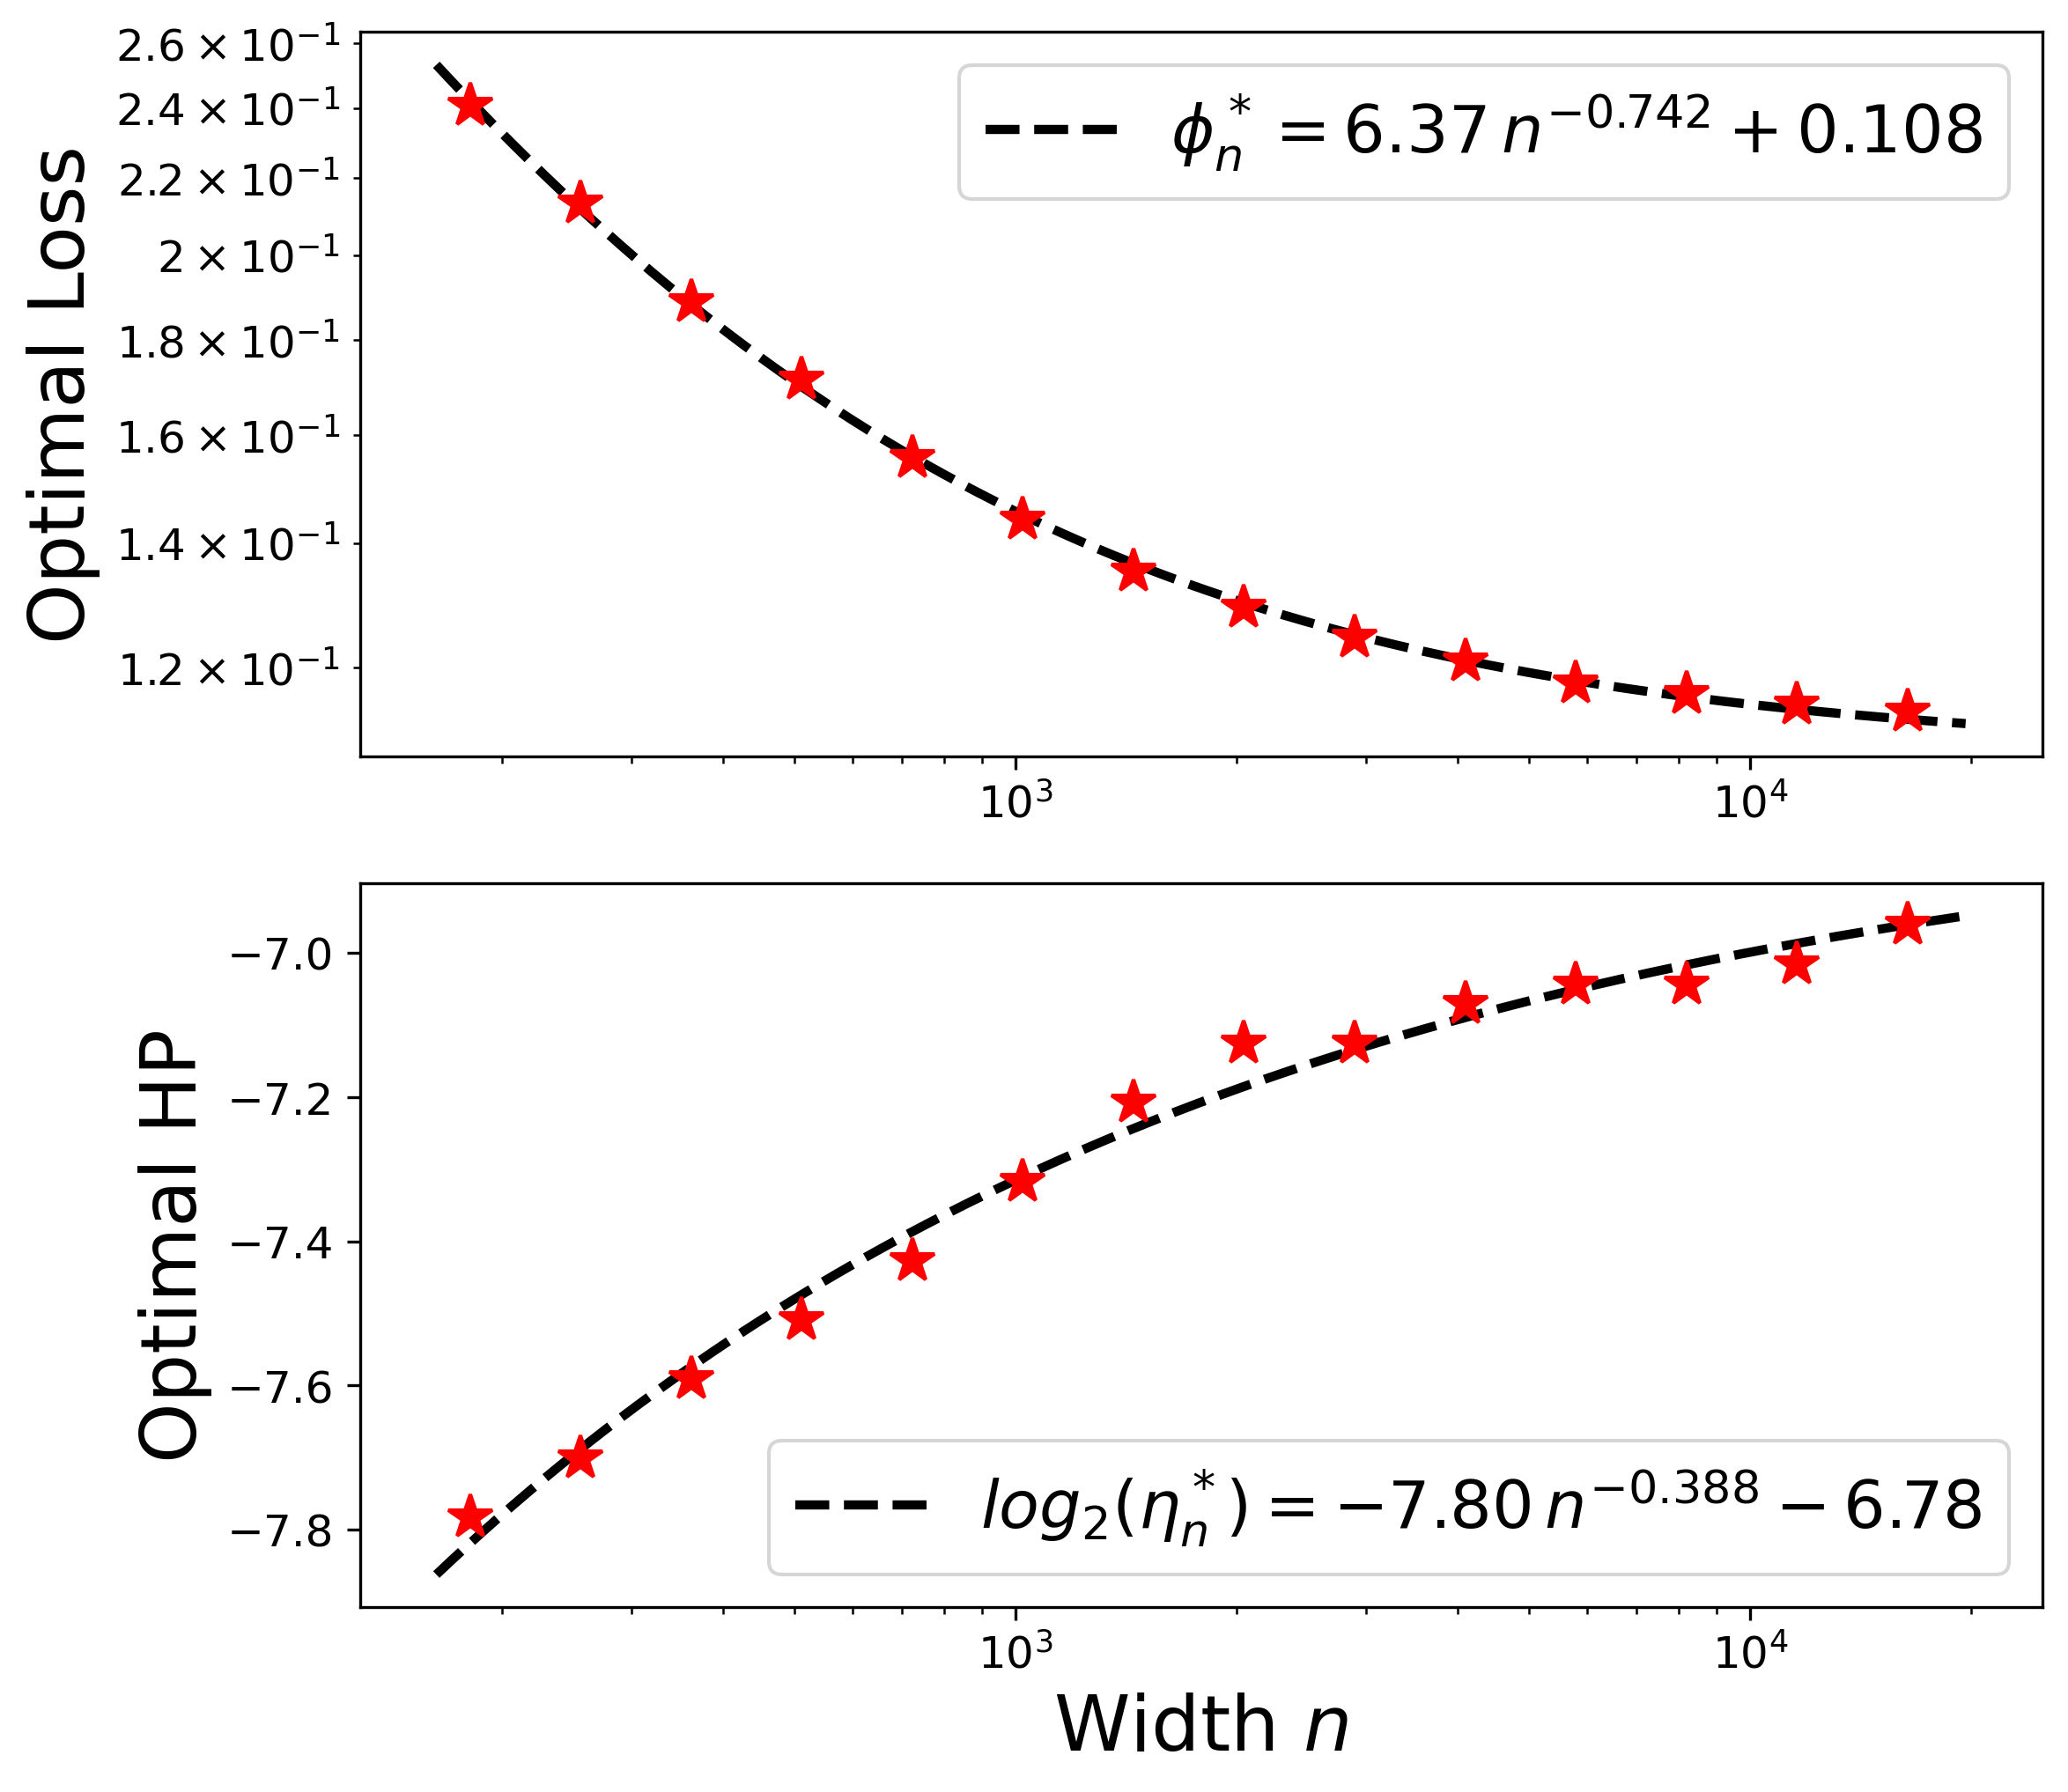
\includegraphics[height=0.65\textwidth]{figures/two_layer_ReLU_rate.png}}  \vspace{-1mm}
\caption{\small Convergence of optimal loss and learning rate.} 
\label{fig:two-layer-ReLU-scaling}
\end{subfigure}%
% \vspace{-1mm} 
\caption{\small Optimal learning rate (validation loss) for two-layer ReLU network to learn the ball indicator function. } 
\vspace{-1.5mm}
\label{fig:two-layer-ReLU} 
\end{figure} 


\paragraph{Slow HP Transfer: Two-layer ReLU Network.} Next we consider a classification setting with a shallow ReLU neural network: $f(\bx) = \sum_{i=1}^n a_i \sigma(\langle \bw_i,\bx\rangle + b_i)$, where we aim to tune the learning rate $\eta$ that minimizes the validation loss. 
We set the target to be the norm indicator function, 
which is a well-studied function that requires a wide two-layer network to approximate \citep{safran2022optimization}, 
\[
y = \mathbbm{1}\big\{\norm{\bx}_2^2 > F_{\chi_d^2}^{-1}(0.5)\big\}, \quad \text{where~ } \textstyle\bx\sim\mathcal{N}(0,\bI_d),
\]
where $F_{\chi_d^2}^{-1}(0.5)$ represents the median of a chi-square distribution with $d$ degrees of freedom. This threshold ensures that the classes are exactly balanced. 
We set $d=2^6, n=2^{14}$, and run the Adam optimizer \citep{kingma2014adam} for $T=2^{14}$ steps with batch size $2^8$ to minimize the binary cross-entropy loss. The initialization and learning rate are set according to $\mu$P \citep{yang2021tensor}. 

In Figure~\ref{fig:two-layer-ReLU-loss} we observe that under $\mu$P, while the optimal learning rate admits a well-defined limit, there is still a visible drift towards the right. Moreover, Figure~\ref{fig:two-layer-ReLU-scaling} illustrates that under a power-law fit, the optimal $\eta$ converges slower than the validation loss, and the estimated scaling $b_n\sim \sqrt{a_n}$ suggests that the HP convergence rate does not beat the agnostic rate from strong convexity. We speculate that the absence of fast transfer in this example is due to the approximation hardness of the target function: achieving low test loss requires exponentially many neurons, and thus polynomial-width dynamics may not accurately track the infinite-width limit and fail to predict the optimal HPs. 
An interesting future direction is to analytically derive the scaling exponents in $a_n,b_n,c_n$ for similar $\mu$P examples and quantify the efficiency of learning rate transfer 
(beyond the definition of weak transfer in Section~\ref{sec:framework}). 

